\section{Galaxy evolution}
\label{sec:evolution}

Galaxy evolution has been explained by many authors [TODO: expand to create a list] \citep{baldry2004quantifying,2006MNRAS.373..469B} by referring to galaxy colour-colour and colour-magnitude diagrams (CMD) \citep[see e.g.][]{2001AJ....122.1861S, 2003ApJ...585L...5H, 2003ApJS..149..289B}. Figure~\ref{fig:CMD1} provides an example of a CMD constructed from SDSS observations of 20,000 nearby galaxies. Gas-rich, star-forming, often disc-like galaxies populate the so-called 'blue cloud' region of the CMD. As gas is consumed through star formation blue cloud galaxies are understood to transition to the redder mainly early-type elliptical quiescent galaxies along the upper left in the 'red sequence' region of the CMD. There is a sparsely populated region separating the blue cloud and red sequence populations often referred to as the 'green valley' region of the CMD  \citep{2004ApJ...608..752B}. In this paper we explore the evolutionary pathway of galaxies in transition between the blue cloud and the red sequence, through the green valley.
It is of interest to note \citet{Mutch_2011} claim that the Milky Way and the Andromeda galaxy M31 are in evolutionary transition due to consumption of cold gas and both lie within the green valley region of the galaxy CMD.

\begin{figure}
	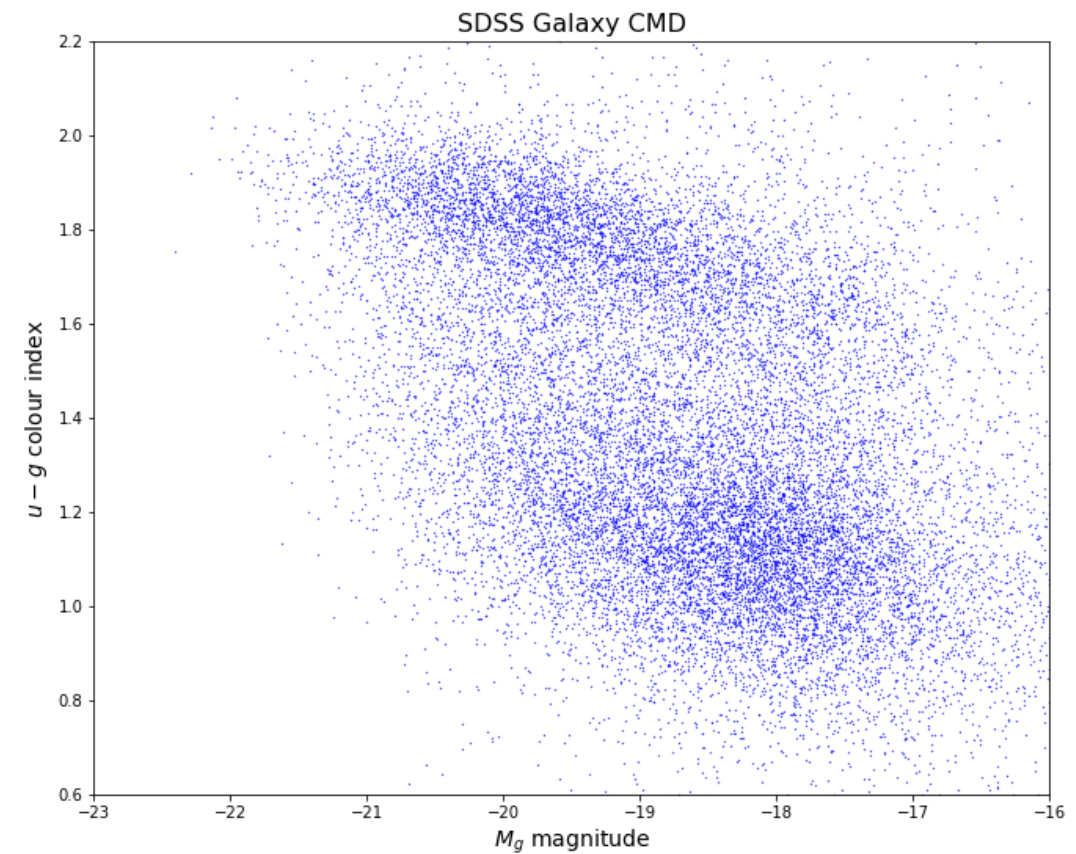
\includegraphics[width=\columnwidth]{images/CMDs/galaxyCMD.PNG}
    \caption{Galaxy colour-magnitude diagram: $u-g$ colour index versus $M_g$ magnitude. The bimodality of the distribution is discussed in the text.}
    \label{fig:CMD1}
\end{figure}